\part{Conclusion}

\chapter{Bilan et perspectives}
Ce travail de thèse s'inscrit dans le cadre de la conception et l'utilisation d'Environnements Informatiques pour l'Apprentissage Humain afin d'aider à l'apprentissage de gestes. Les EIAH dédiés à l'apprentissage de gestes existants sont souvent limités dans leur capacité à être réutilisés dans des contextes applicatifs variés. La recherche de la généricité d'un tel système doit se faire dès sa conception, et il doit en particulier être en mesure de proposer une intégration aisée de la connaissance experte. Ainsi, notre objectif a été de créer un EIAH générique au regard du domaine considéré, permettant d'assister l'apprenant dans sa tâche d'apprentissage du geste, et l'enseignant dans son analyse du mouvement et sa restitution à l'apprenant.

\section{Synthèse des contributions}
Nous avons proposé un EIAH dédié à l'apprentissage de gestes et conçu de manière à être générique. Cet EIAH est divisé en deux grandes parties. La première permet d'importer, de filtrer et d'extraire des descripteurs à partir de fichiers de mouvements au format BVH (BioVision Hierarchy). La chaîne de traitement proposée n'agit que sur les descripteurs extraits du mouvement, et non sur le mouvement en lui-même, corrigeant ainsi les irrégularités directement sur les valeurs des descripteurs. En effet, la correction de ces erreurs en amont nécessiterait de faire des hypothèses quant aux causes des problèmes présents au sein des données. Particulièrement adaptée aux gestes possédant au moins une accélération soudaine (comme les gestes de lancers), elle permet également de ne conserver automatiquement qu'une partie du mouvement, appelée \textit{Motion of Interest} (\textit{MoI}), afin d'éviter une segmentation manuelle dans le cas où plusieurs gestes similaires sont à traiter. L'extraction des descripteurs requis se fait à l'aide de structures de données internes adaptées à l'export au format JSON.

La deuxième partie du système permet la comparaison des mouvements de l'apprenant à ceux de l'expert. L'affichage des différences entre ces mouvements apporte une aide à l'enseignant conseillant l'apprenant en vue de l'amélioration de son geste. Le système permet d'afficher et de quantifier l'importance des défauts du geste de l'apprenant, et permet d'établir une stratégie de conseil en ciblant les défauts à corriger en premier. Les données de l'expert, servant de base pour la comparaison, peuvent être regroupées à l'aide de techniques de clustering, afin d'identifier les propriétés des groupes constitués : (i) majoritairement de gestes acceptables ou (ii) majoritairement des gestes non acceptables. La visualisation des données de l'apprenant et de l'expert permet de rapidement déterminer quels sont les défauts les plus proéminents dans les gestes de l'apprenant, et ainsi de proposer une correction adaptée. L'intégration des conseils donnés par l'expert pour chacun des défauts identifiés est également possible et permet, dans une certaine mesure, d'utiliser le système en autonomie.

Les expérimentations menées ont permis de tester plusieurs aspects du système. La première expérimentation, concernant le lancer d'une balle dans deux corbeilles différentes, a montré qu'il était possible de séparer les données à l'aide de descripteurs basés sur la vitesse dans le cas de ce lancer. La deuxième expérimentation, utilisant le geste du Bottle Flip Challenge, cherchait à vérifier s'il était possible d'obtenir une séparation correspondant au degré de réussite du geste, tout en utilisant des descripteurs basés sur la vitesse. Les résultats n'ont pas été concluants sur le degré de réussite, bien qu'un regroupement acceptable a été obtenu. La troisième expérimentation, portant sur le lancer de fléchettes, avait pour objectif de vérifier la capacité du système à être utilisé afin de prodiguer des conseils pertinents au regard des défauts du geste des apprenants. Les participants à l'expérimentation ont été séparés en trois groupes : (a) un groupe où seul l'expert analysait le geste et donnait des conseils pour son amélioration, (b) un groupe où l'expert pouvait s'appuyer, si besoin, sur le système afin de donner des conseils et (c) un groupe où l'expert restituait les conseils donnés par le système. L'analyse s'est effectuée sous deux angles principaux : l'amélioration de l'objectif du geste (distance des fléchettes par rapport au centre), et l'amélioration du geste en lui-même (distance des données de l'apprenant par rapport au centroïde des bon gestes de l'expert). Ainsi, bien que la précision n'ait pas augmenté, une amélioration du geste a été constatée sur chaque aspect du geste considéré (en termes de correction de défauts), ainsi que sur le geste dans sa globalité au fur et à mesure de l'expérimentation. L'utilisation du système par un expert pour l'assister dans sa tâche d'enseignement a également conduit à une amélioration du geste. Cependant, aucune différence significative au regard de l'amélioration du geste n'a été obtenue entre les différents groupes, ne permettant pas ainsi de conclure quant à la valeur ajoutée apportée par le système dans le cadre d'une session courte d'apprentissage de cette tâche.

Ce travail présente des limites, et ouvre la porte à de nombreuses perspectives d'ingénierie et de recherche.


\section{Limites des travaux et du système MLA}
Une première limite du travail réside dans le manque d'interface graphique pour l'utilisation de la plateforme \textit{MLA}. En l'état, la sélection du dossier contenant les données de l'apprenant pour la phase de pré-traitement se fait directement au sein du code. Ainsi, il est nécessaire de re-compiler le code pour chaque nouvelle personne. De plus, la sélection des données des personnes à traiter, ainsi que les descripteurs associés aux défauts à analyser se font également à la main dans le code Python. Bien qu'une compilation ne soit pas nécessaire pour cet aspect, ce processus est tout autant fastidieux. Une interface graphique, soit séparée selon les deux parties du système, soit unifiée, permettrait de grandement faciliter la manipulation de l'outil, en limitant les compétences techniques demandées à l'utilisateur. Une perspective pour combler cette limite actuelle est proposée dans la section suivante.

La pertinence des indicateurs à visualiser (descripteurs du mouvement, métrique de clustering, \textit{etc.}), ainsi que la visualisation proposée à l'expert ou l'apprenant reste à déterminer, par le biais d'expérimentation avec des personnes non-expertes dans l'utilisation du système. La visualisation actuellement proposée répond aux besoins d'observations de l'expérimentation réalisée, mais sa généralisation à d'autres domaines applicatifs n'est pas garantie.

L'utilisation de la combinaison Perception Neuron pour la capture des données nécessite des étapes de filtrage des données, afin qu'elles soient exploitables. Bien que les techniques de filtrage des données mises en places permettent d'obtenir des données acceptables dans le contexte des expérimentations réalisées, ces méthodes n'ont pas été conçues pour traiter n'importe quels types de gestes. L'utilisation de méthodes de captation de meilleure qualité permettrait d'obtenir des données plus précises, et de s'affranchir des filtrages mis en place.

Le faible nombre de lancers, ainsi que la réalisation d'une seule séance d'apprentissage du geste, pour le lancer de fléchettes ne permet pas de juger correctement de la capacité du système à assister un apprenant ou un expert sur le long terme. En effet, dans une situation d'apprentissage classique, l'apprentissage s'effectue sur plusieurs séances, et le nombre de lancers par séance est beaucoup plus conséquent.

\section{Perspectives sur le projet MLA}

\subsection{Interface graphique}
La partie en charge du pré-traitement des données doit bénéficier d'une interface graphique, afin de choisir quels descripteurs sont à extraire, ainsi que les paramètres des différents algorithmes : filtrage, mouvement à extraire (possibilité de directement choisir sur un graphique), \textit{etc.} Cette partie nécessite pour l'instant des connaissances (i) sur les données de mouvement, (ii) scientifiques pour le choix des paramètres des algorithmes et des filtres et (iii) techniques pour la modification de ces paramètres. En proposant une visualisation du résultat du filtrage et du mouvement à extraire, il est possible de diminuer la complexité d'utilisation du système et ainsi permettre à des non-experts de modifier ces paramètres.

Dans l'optique de faciliter l'utilisation du système \textit{MLA}, une première maquette d'une interface graphique pour la partie donnant des retours sur le mouvement a été réalisée (Fig. \ref{fig:MLA_GUI_mockup}). La configuration de l'analyse se fait selon l'ordre établi auparavant, à savoir descripteur puis articulation.

\begin{figure}[h]
    \centering
    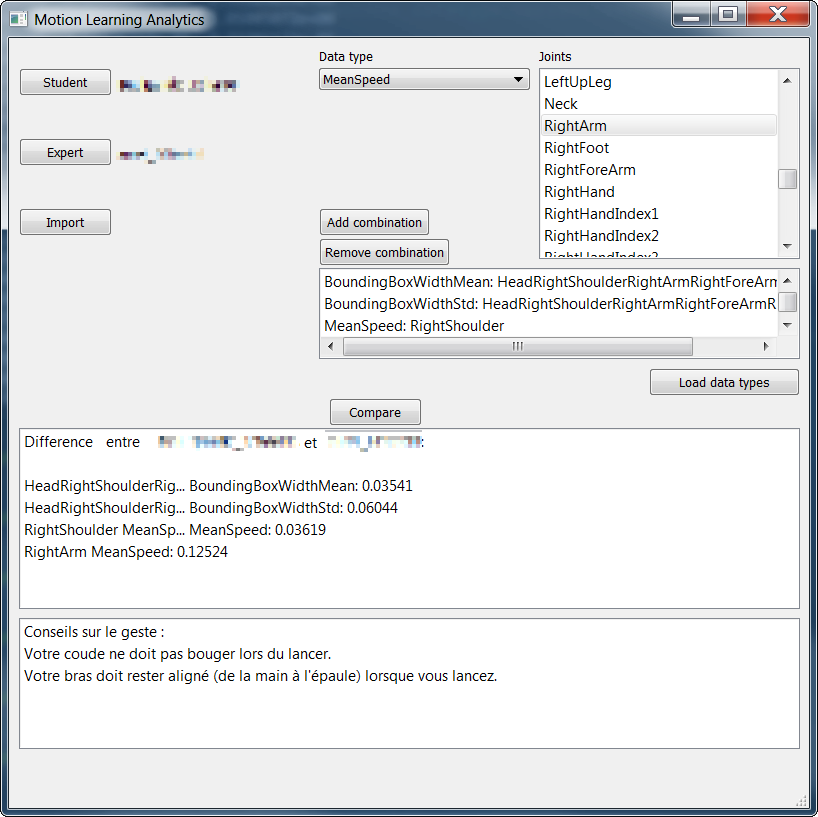
\includegraphics[width=\textwidth]{pictures/MLA_GUI_mockup.png}
    \caption[Une première itération de l'interface graphique des modules d'analyse de MLA]{Une première itération de l'interface graphique des modules d'analyse de MLA. Les types de données possibles, ainsi que les articulations disponibles pour les mouvements capturés sont directement extraits des données retournées par les modules de pré-traitements au format \textit{JSON}.}
    \label{fig:MLA_GUI_mockup}
\end{figure}

L'intégration des différents retours proposés à l'enseignant dans les dernières versions de \textit{MLA} (visualisation de la distance des données de l'apprenant par rapport aux données de l'expert, métriques calculées sur les groupements obtenus, \textit{etc.}) sera l'objet d'une autre itération de cette interface.

\subsection{Explication des données non-alignées de l'apprenant}
Une des difficultés d'interprétation du retour visuel fourni à l'expert se situe dans le cas où les données de l'apprenant ne sont pas situées dans un des clusters de mouvements de l'expert et qu'elles n'appartiennent pas au trapèze formé par les deux clusters (Fig. \ref{fig:non_aligned_default}, partie verte claire).

\begin{figure}[h]
    \centering
    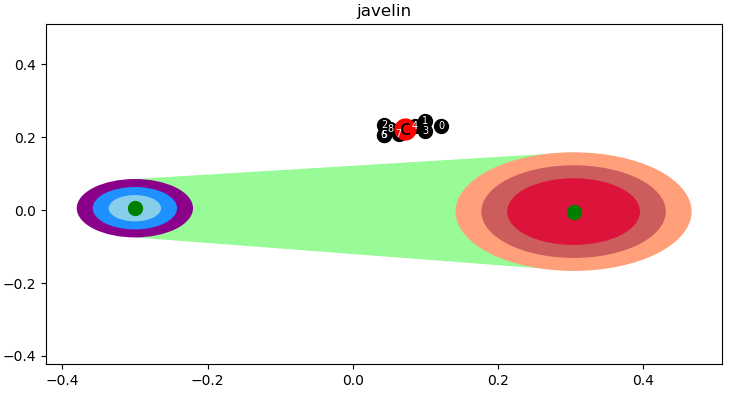
\includegraphics[width=\textwidth]{pictures/non_aligned_default.png}
    \caption[Un exemple de non-alignement des données de l'apprenant par rapport à celles de l'expert]{Dans cet exemple, on peut constater que les données de l'apprenant ne se situent pas dans le trapèze formé par les deux clusters de l'expert. L'explication en détail du défaut est difficile dans ce cas.}
    \label{fig:non_aligned_default}
\end{figure}

Cette différence, lorsque les données utilisées sont de dimension 2, peut s'expliquer visuellement, sous réserve de posséder les connaissances scientifiques nécessaires à l'analyse de ces données. En effet, dans ce cas, il est possible d'obtenir directement quelles sont les différences entre les valeurs des descripteurs de l'expert et ceux de l'apprenant. Cependant, lorsque la dimensionnalité des données est plus élevée, le non-alignement des données de l'apprenant avec celles de l'expert ne peut s'expliquer aussi facilement. En effet, l'affichage des données est actuellement réalisé sur un graphique possédant uniquement deux dimensions. Il serait possible d'étendre cette visualisation en 3D, mais le problème se pose toujours pour les données de dimension supérieure. Il est donc nécessaire de réduire la dimensionnalité des données lorsque celle-ci est supérieure à deux. Cette étape implique une réduction des données, et les valeurs représentées sur les deux axes du graphique ne peuvent être corrélées à une caractéristique du geste si elle est représentée par un vecteur à plus de deux dimensions dans le système actuel. En effet, elles peuvent être issues de la fusion de plusieurs caractéristiques possédant un pouvoir de discrimination entre les mouvements plus faible, ou encore de la suppression de certaines de ces caractéristiques, en fonction de la méthode choisie.

Ainsi, une des pistes de travail est d'étudier la sémantique et l'origine des données non-alignées. L'objectif sera de proposer une comparaison des différents descripteurs utilisés. Une première étape réside dans le calcul de la moyenne des écarts de chaque dimension des données de l'apprenant avec chaque dimension des données de l'expert étiquetée comme geste cible, afin d'obtenir une valeur correspondant à la différence brute entre ces données. Ainsi, il serait possible de proposer une explication sur les différences entre les gestes de l'expert et ceux de l'apprenant. La deuxième étape serait ensuite de travailler sur le sens de cette différence, autant pour l'expert que pour l'apprenant. Cette étape implique d'être capable de donner une sémantique pédagogiquement utile.

\subsection{Création de nouveaux descripteurs à l'aide d'un système fondé sur des patrons de conception}

% Wesh alors là ma gueule autant j'ai l'idée générale, autant j'ai Z E R O idée de comment implémenter ça. Mais j'pense que c'est une bonne idée.

L'implémentation des descripteurs élémentaires proposés au Chapitre \ref{chap:descripteurs} permet de limiter le nombre de descripteurs à implémenter, tout en permettant de couvrir des besoins d'observation et d'analyse variés. En pratique, il est possible que les besoins de l'expert ne concernent qu'une dimension d'un descripteur élémentaire, ou au contraire une combinaison de plusieurs de ces descripteurs. Par exemple, la hauteur de la hanche est la dimension verticale du descripteur position de la hanche. Une des solutions possibles est de proposer l'extraction de composantes de descripteurs existants (la valeur en $x$ de du vecteur vitesse par exemple), ou la fusion de descripteurs déjà implémentés. Cette méthode pourrait s'appuyer sur une approche basée sur un langage créé pour ce cas d'usage, comme présentée dans le chapitre \ref{chap:descripteurs}, section \ref{sec:class_descr} : en spécifiant un ou une combinaison de descripteurs, l'intervalle ou les postures sur lesquelles il est choisi, il serait possible de créer de nouveaux descripteurs. Plusieurs exemples :

\begin{framed}
\begin{lstlisting}[breaklines]
DESCRIPTOR Hauteur hanche: POSITION_ALL[2]
\end{lstlisting}
\end{framed}
pour la hauteur de la hanche (valeur en \textit{y}) calculée sur tout le mouvement.\\

\begin{framed}
\begin{lstlisting}[breaklines]
DESCRIPTOR Vitecceleration: SPEED_ALL[2] + ACCELERATION_ALL[1]
\end{lstlisting}
\end{framed}
pour calculer l'addition de la composante en $y$ de la vitesse et de la composante en $x$ de l'accélération.\\

\begin{framed}
\begin{lstlisting}[breaklines]
DESCRIPTOR Vitecceleration constante: SPEED_ALL[3] * CONSTANT_ACCELERATION_SPECIFIC[15][1]
\end{lstlisting}
\end{framed}
permettrait de calculer la vitesse sur l'axe $z$ sur tout le mouvement, multipliée par la valeur d'accélération sur l'axe \textit{x} de la frame 15.


\subsection{Expérimentation à plus grande échelle}
Les expérimentations présentées dans ce manuscrit ont pris place dans un espace de temps très court pour chaque participant. Ainsi, pour le \textit{Bottle Flip Challenge}, les cent lancers ont été réalisés à la suite. Pour le lancer de fléchettes, seuls trente-six lancers ont été réalisés par personne, ce qui est très peu au regard d'une séance d'apprentissage classique. Dans ces conditions, l'amélioration du geste peut être marginale, voire inexistante, à cause de la fenêtre de temps très réduite pour l'évaluation. En conséquence, le système devra être testé sur une multitude de séances d'entraînement, de durée plus conséquente, afin de prouver ou non sa capacité à assister l'expert dans son évaluation du geste de l'apprenant dans un contexte d'apprentissage réel. De plus, une telle évaluation permettrait de tester l'utilisabilité du système au travers des interfaces à développer évoquées précédemment.

\subsection{Expérimentation d'apprentissage en autonomie}
Il est également intéressant de se pencher sur l'utilisation de ce système en autonomie, c'est-à-dire un apprenant seul conseillé par le système. L'intégration des retours de l'expert, en fonction des différences du geste de l'apprenant par rapport à ceux de l'expert, pourra s'effectuer en même temps que la sélection des descripteurs à observer. Le système pourra donc être utilisé en autonomie par l'apprenant. L'analyse de la progression du geste à travers une utilisation en autonomie et la comparaison avec la progression en présence d'un expert peut être à même de donner des pistes d'améliorations pour les conseils donnés par le système. La prolongation de l'expérimentation du lancer de fléchettes sur plusieurs séances pour chaque personne permettrait de vérifier l'évolution du geste, ainsi que la rapidité de l'évolution du geste, au fur et à mesure des séances d'apprentissage, et permettrait ainsi de comparer ces évolutions entre les différents groupes (expert  / expert assisté du système / système).

\subsection{Extension des expérimentations à d'autres gestes}
Bien que pensé pour être générique dès sa conception, la généricité du système devra être améliorée afin de répondre à plusieurs cas d'études impliquant des gestes différents dans plusieurs domaines. Les domaines applicatifs retenus devront cependant respecter plusieurs critères :
\begin{itemize}
	\item Existence d'expertise dans le domaine : la présence d'un expert reconnu (soit par des diplômes, soit par ses pairs) permet de s'assurer de l'existence d'une connaissance experte.
	\item Possibilité de formaliser la connaissance experte en descripteurs : cette étape est cruciale, car c'est elle qui déterminera quelles seront les caractéristiques du geste à analyser. La sélection des descripteurs à calculer et à utiliser se fait à cette étape, avec l'aide de l'expert.
	\item Séances d'apprentissage contenant les mêmes gestes : la similarité des gestes effectués entre les différentes séances d'apprentissage permet d'assurer la continuité des conseils donnés.
	\item Possibilité d'acquérir suffisamment de données au cours d'une seule séance d'apprentissage : le système nécessite un certain nombre de gestes (autant de la part de l'expert que de celle de l'apprenant) afin de proposer un retour visuel représentatif de la performance de l'apprenant. Il peut néanmoins être intéressant de tester le système sur une donnée de l'apprenant à la fois, afin de vérifier si la visualisation des défauts, ainsi que les conseils donnés par le système restent pertinents.
\end{itemize}

\subsection{Clustering récursif}
Une piste explorée, mais non concrétisée, au cours de la thèse a été celle de l'utilisation d'algorithmes de clustering de manière récursive sur chaque groupe obtenu lors d'un premier clustering. Cette idée provient de la volonté d'obtenir une séparation des données en groupes de données correspondants aux gestes réussis et aux gestes ratés. Au terme de l'expérimentation du \textit{Bottle Flip Challenge}, il n'a pas été possible d'obtenir cette séparation. Cependant, une hypothèse soulevée était que la granularité de la séparation (en deux groupes) n'était pas assez fine et qu'il existait différents stratégies ou groupes de mouvements, possédant des caractéristiques différentes, conduisant au succès de la tâche. L'observation des caractéristiques les plus discriminantes entre ces deux groupes a montré que la séparation se faisait sur la vitesse du lancer. De là est venue l'idée d'appliquer récursivement un algorithme de clustering sur les deux groupes obtenus, afin de vérifier si, au sein de ces groupes, il était possible d'obtenir un groupement des données qui correspondait au degré de réussite du geste. Ainsi, nous faisons l'hypothèse qu'il est possible d'obtenir un ensemble défini de sous-groupes composés majoritairement de gestes réussis, ou  majoritairement de gestes ratés. Un travail de recherche devra être conduit pour confirmer ou infirmer cette hypothèse.

La méthode testée se base pour l'instant sur une approche semi-supervisé d'apprentissage automatique. En effet, bien que l'objectif à terme soit d'utiliser des métriques calculées sur les clusters afin de déterminer si les sous-groupes obtenus sont corrects, le critère d'arrêt actuel utilise le taux de gestes du même type au sein des sous-groupes obtenus. Dans notre cas, l'étiquetage des données correspondant à la réussite ou non du geste.

En partant initialement d'un ensemble constitué de la totalité des données, l'algorithme effectue plusieurs clustering sur ces données, avec un nombre $k = 2, 3, 4, \ldots, 8$ de clusters. Seul le meilleur clustering, au sens du Silhouette Score, est conservé. Pour chaque sous-groupe ainsi obtenu, la répartition des données en son sein est alors calculée. Un sous-groupe est considéré comme homogène dès lors qu'il contient au moins 75\% de gestes du même type (réussi ou raté), et l'algorithme ne fait pas de passe supplémentaire dessus. Enfin, lorsqu'un groupe ne contient plus que quatre données, aucun clustering n'est appliqué dessus.

Les premiers résultats obtenus ont montrés qu'il était possible d'obtenir un taux de même geste au sein des clusters supérieur ou égal au seuil défini. Le travail de recherche devra se concentrer dans un premier temps sur l'analyse de la pertinence des paramètres choisis : taille minimale du sous-groupe, seuil de répartition des gestes, algorithmes utilisés. Un travail de recherche doit ensuite être effectué afin d'analyser les spécificités communes des gestes entre eux, au sein de chaque sous-groupe obtenu, afin de vérifier si (i) les propriétés communes des gestes au sein de chaque sous-groupe sont pertinentes au regard du geste considéré, et si (ii) des sous-groupes ont en communs ces propriétés, afin de les réunir dans une approche ascendante, analogue au clustering hiérarchique.